\chapter{Results}\label{chap:results}

\section{Experimental Results}
\label{sec:experimental_results}

The experimental forming limits obtained on the high-throughput test bench described in Chapter~\ref{chap:experimental_campaign} are reported in this section. They provide the reference against which the numerical forming limit curves of the later sections are compared.

\subsection{Influence of Material Orientation}
\label{sec:orientation_influence}

A dedicated subset of the campaign was used to isolate the influence of material orientation on the experimentally determined forming limits. For every sheet thickness (A--D), the \SI{100}{\milli\meter} hemispherical punch was tested with the specimen long axis aligned both with the rolling direction (RD, configuration \texttt{E0\_RM00\_000}) and with the transverse direction (TD, configuration \texttt{E0\_RM00\_090}). The configuration label encodes the punch and orientation: the trailing \texttt{000} and \texttt{090} denote the in-plane angle $\alpha$ between the specimen long axis and the rolling direction, so that \texttt{E0\_RM00\_000} corresponds to RD ($\alpha = \SI{0}{\degree}$) and \texttt{E0\_RM00\_090} to TD ($\alpha = \SI{90}{\degree}$). All other parameters (punch diameter, specimen widths, and test bench settings) are held identical between the two orientations, so that any difference in the resulting forming limits can be attributed to anisotropy alone.

For each orientation and thickness, two complete campaigns of seven specimen widths were performed, and the forming-limit points reported here are the mean over the two campaigns. Averaging over two independent sets reduces the influence of anomalies that a single set may carry, such as local material defects, specimen handling or operator errors, or other test-specific outliers, so that the reported curve reflects the representative material response rather than the particular condition of one set. The limit points themselves were determined from the DIC strain fields using the section-line (DIN) method of DIN EN ISO 12004-2~\cite{ISO120042}, in which strain profiles are evaluated along section lines placed across the necking zone and the limit strains are recovered from an inverse best-fit of these profiles. The same evaluation pipeline used throughout this work was applied, enforcing both the robustness and accuracy selection criteria. Figure~\ref{fig:rd_vs_td} overlays the resulting RD and TD forming limit curves for the four thicknesses.

\begin{figure}[H]
    \centering
    \begin{subfigure}[t]{0.49\textwidth}
        \centering
        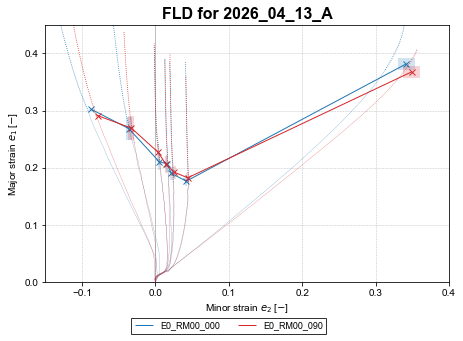
\includegraphics[width=\textwidth]{report/img/RD_vs_TD_A.png}
        \caption{Material A ($t = \SI{1.2}{\milli\meter}$).}
        \label{fig:rd_vs_td_a}
    \end{subfigure}
    \hfill
    \begin{subfigure}[t]{0.49\textwidth}
        \centering
        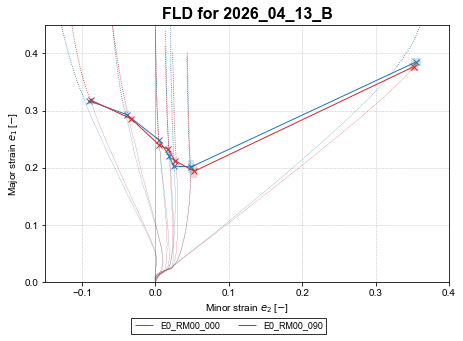
\includegraphics[width=\textwidth]{report/img/RD_vs_TD_B.png}
        \caption{Material B ($t = \SI{1.5}{\milli\meter}$).}
        \label{fig:rd_vs_td_b}
    \end{subfigure}

    \vspace{0.5em}

    \begin{subfigure}[t]{0.49\textwidth}
        \centering
        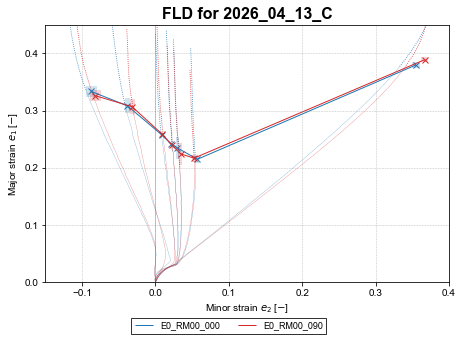
\includegraphics[width=\textwidth]{report/img/RD_vs_TD_C.png}
        \caption{Material C ($t = \SI{2.0}{\milli\meter}$).}
        \label{fig:rd_vs_td_c}
    \end{subfigure}
    \hfill
    \begin{subfigure}[t]{0.49\textwidth}
        \centering
        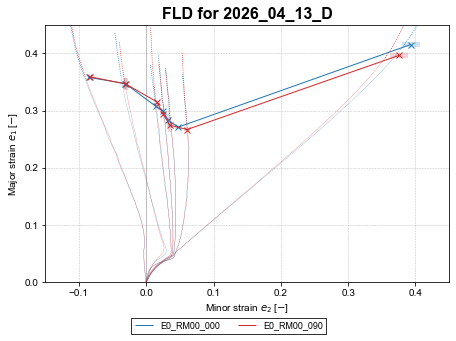
\includegraphics[width=\textwidth]{report/img/RD_vs_TD_D.png}
        \caption{Material D ($t = \SI{3.0}{\milli\meter}$).}
        \label{fig:rd_vs_td_d}
    \end{subfigure}
    \caption{Comparison of forming limit curves measured in the rolling direction (\texttt{E0\_RM00\_000}, RD) and the transverse direction (\texttt{E0\_RM00\_090}, TD) for the \SI{100}{\milli\meter} punch, shown for the four sheet thicknesses A--D. Each curve is the mean of two complete campaigns, with limit points evaluated using the DIN section-line method (DIN EN ISO 12004-2) under the robustness and accuracy criteria.}
    \label{fig:rd_vs_td}
\end{figure}

Across all four thicknesses the RD and TD forming limit curves are essentially coincident. The two orientations follow the same trajectory from the uniaxial branch through the plane-strain minimum and into the biaxial branch, and the residual differences between them remain within the scatter of the underlying campaigns. The separation between the RD and TD curves is consistently smaller than the spread observed between the two repeated campaigns of a single orientation, so it cannot be distinguished from experimental repeatability. No systematic trend with thickness is observed: the orientations do not diverge more strongly for the thinner sheets (A, B) than for the thicker ones (C, D).

These results indicate that, for the AA5754 sheet material and thickness range investigated here, in-plane material orientation has no measurable influence on the forming limits. This justifies restricting the remaining punch-diameter campaigns to the rolling direction and supports the use of an in-plane isotropic description of the forming limits in the numerical model developed in Chapter~\ref{chap:numerical_model}.

\subsection{Punch Diameter, Sheet Thickness, and the Evaluation Window}
\label{sec:punch_thickness}

The second experimental study varies the punch diameter ($\varnothing$40, 60, 80, and 100\,mm) across the four sheet thicknesses (A--D) to expose the coupling between punch geometry and sheet thickness. Physically, a smaller punch superimposes more bending on the membrane stretch and produces a steeper through-thickness strain gradient, which stabilises the deformation against localised necking. The magnitude of this effect scales with the ratio $t/R$ of sheet thickness to punch radius. Two trends are therefore expected: the forming limit curve should rise as the punch diameter decreases, and the spread between punch diameters should widen with increasing thickness, since $t/R$ grows fastest for the smallest punch on the thickest sheet.

Figure~\ref{fig:flc_norm} shows the forming limit curves obtained with the standard ISO~12004-2 evaluation, that is, the intersection-line method of Section~\ref{sec:din_method} using the window width of Eq.~\eqref{eq:din_window} with its calibration constant of $10$. For the 100, 80, and 60\,mm punches the expected ordering is recovered, but the 40\,mm punch does not follow it: its limit curve lies far above the others, by a margin that grows with thickness and that is too large to be attributed to the $t/R$ curvature effect alone. Because all curves in a given diagram originate from the same material and thickness, this incoherence points to the evaluation rather than to the material response. The standard window is calibrated for the $\varnothing$100\,mm Nakazima geometry, whereas the 40\,mm punch produces a much narrower neck, so a window sized for the standard punch no longer matches the strain field to which it is applied.

\begin{figure}[H]
    \centering
    \begin{subfigure}[t]{0.49\textwidth}
        \centering
        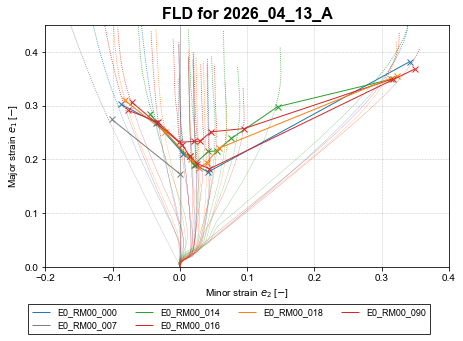
\includegraphics[width=\textwidth]{report/img/FLC_norm_A.png}
        \caption{Material A ($t = \SI{1.2}{\milli\meter}$).}
        \label{fig:flc_norm_a}
    \end{subfigure}
    \hfill
    \begin{subfigure}[t]{0.49\textwidth}
        \centering
        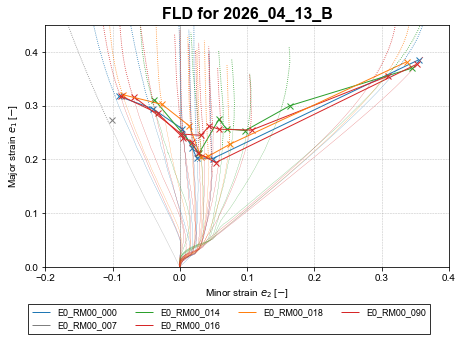
\includegraphics[width=\textwidth]{report/img/FLC_norm_B.png}
        \caption{Material B ($t = \SI{1.5}{\milli\meter}$).}
        \label{fig:flc_norm_b}
    \end{subfigure}

    \vspace{0.5em}

    \begin{subfigure}[t]{0.49\textwidth}
        \centering
        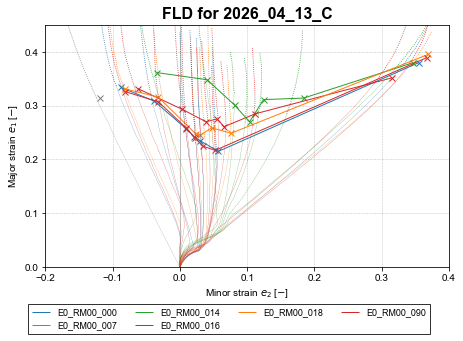
\includegraphics[width=\textwidth]{report/img/FLC_norm_C.png}
        \caption{Material C ($t = \SI{2.0}{\milli\meter}$).}
        \label{fig:flc_norm_c}
    \end{subfigure}
    \hfill
    \begin{subfigure}[t]{0.49\textwidth}
        \centering
        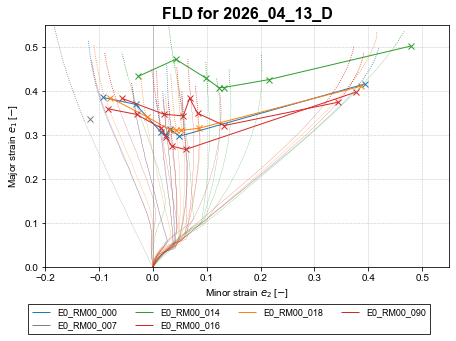
\includegraphics[width=\textwidth]{report/img/FLC_norm_D.png}
        \caption{Material D ($t = \SI{3.0}{\milli\meter}$).}
        \label{fig:flc_norm_d}
    \end{subfigure}
    \caption{Forming limit curves for the four punch diameters (\texttt{014}/40, \texttt{016}/60, \texttt{018}/80, \texttt{000}/100\,mm) obtained with the standard ISO~12004-2 window (Eq.~\eqref{eq:din_window}, constant $=10$), for the four sheet thicknesses A--D. The 40\,mm punch (green) departs from the expected ordering by an implausibly large margin that grows with thickness.}
    \label{fig:flc_norm}
\end{figure}

The intersection-line method exposes two fixed length-scale parameters: the spacing between intersection lines ($2$\,mm) and the constant factor of $10$ in the window width of Eq.~\eqref{eq:din_window}. These correspond to two physically distinct scales. The fitting window is governed by the extent of the strained dome, which scales with the punch diameter $D$, whereas the excluded near-crack zone is governed by the neck width, which scales with the sheet thickness $t$. The fixed constant captures neither. A minimal, norm-consistent generalisation replaces the constant with $D/10$, so that the window width becomes $\omega = (D/10)\,[1 + \bar{\varepsilon}_2/\bar{\varepsilon}_1]$ and reduces to the standard value for the $\varnothing$100\,mm punch ($100/10 = 10$). Figure~\ref{fig:flc_pscaled} shows the limit curves re-evaluated with this punch-scaled window. Scaling the window with the punch diameter markedly shifts the extracted 40\,mm limit, which confirms that its position under the standard evaluation is governed largely by the window choice rather than by the material.
% TODO(andre): confirm and state precisely whether the D/10 window restores the expected
% 40 > 60 > 80 > 100 ordering, and for which thicknesses it holds. The intersection-line
% spacing (currently fixed at 2 mm) was also varied; describe that variant here if it is kept.

\begin{figure}[H]
    \centering
    \begin{subfigure}[t]{0.49\textwidth}
        \centering
        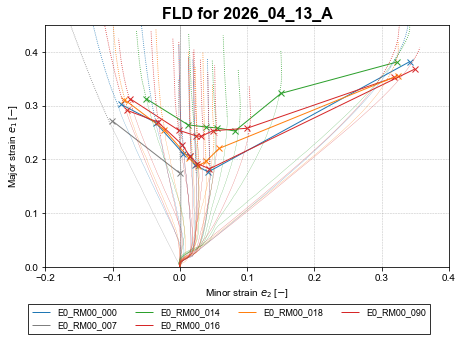
\includegraphics[width=\textwidth]{report/img/FLC_pscaled_A.png}
        \caption{Material A ($t = \SI{1.2}{\milli\meter}$).}
        \label{fig:flc_pscaled_a}
    \end{subfigure}
    \hfill
    \begin{subfigure}[t]{0.49\textwidth}
        \centering
        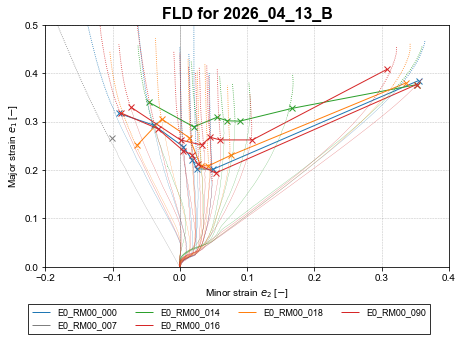
\includegraphics[width=\textwidth]{report/img/FLC_pscaled_B.png}
        \caption{Material B ($t = \SI{1.5}{\milli\meter}$).}
        \label{fig:flc_pscaled_b}
    \end{subfigure}

    \vspace{0.5em}

    \begin{subfigure}[t]{0.49\textwidth}
        \centering
        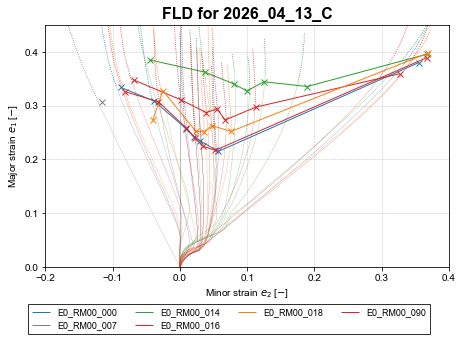
\includegraphics[width=\textwidth]{report/img/FLC_pscaled_C.png}
        \caption{Material C ($t = \SI{2.0}{\milli\meter}$).}
        \label{fig:flc_pscaled_c}
    \end{subfigure}
    \hfill
    \begin{subfigure}[t]{0.49\textwidth}
        \centering
        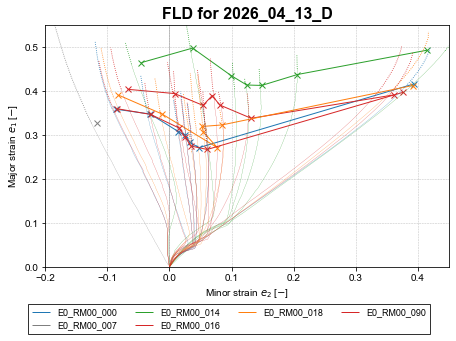
\includegraphics[width=\textwidth]{report/img/FLC_pscaled_D.png}
        \caption{Material D ($t = \SI{3.0}{\milli\meter}$).}
        \label{fig:flc_pscaled_d}
    \end{subfigure}
    \caption{Forming limit curves re-evaluated with a punch-scaled window ($\omega = (D/10)\,[1 + \bar{\varepsilon}_2/\bar{\varepsilon}_1]$), for the four sheet thicknesses A--D. The constant of the standard window (Eq.~\eqref{eq:din_window}) is replaced by $D/10$, recovering the norm for the $\varnothing$100\,mm punch.}
    \label{fig:flc_pscaled}
\end{figure}

These observations indicate that the ISO~12004-2 evaluation, calibrated for a single standardised punch, cannot be transferred unchanged to a campaign that varies the punch diameter: the extracted 40\,mm limit reflects the fixed window as much as the material response. The window width and, by the same argument, the intersection-line spacing should be made tunable and geometry-aware, scaling with the punch diameter and the sheet thickness respectively. The $D/10$ rule is a first, deliberately simple candidate. A defensible parameter choice additionally requires verifying that the extracted limit is insensitive to the window in the neighbourhood of the selected value (a convergence criterion), and cross-validating against the window-independent criteria of Sections~\ref{sec:vh_method} and~\ref{sec:minstoughton_method} (Volk \& Hora and Min--Stoughton). This validation is left to future work.

\section{Framework Outputs and Configuration Coverage}

The results chapter focuses on the implemented numerical workflow and its
interfaces to the experimental campaign and identification framework. For each
selected configuration, the pipeline creates the Abaqus model, submits the
solver job on Euler, runs ODB-based post-processing, and synchronises structured
result artefacts. The same interface is used for Nakazima, Marciniak, and
Punch-in-Punch simulations, so that specimen width, sheet thickness, punch
radius, punch travel, material orientation, mass scaling, and mesh refinement
can be varied without changing the post-processing schema.

Each completed simulation produces the same set of data products:
\texttt{punch\_fd.csv}, \texttt{energy\_data.csv}, \texttt{strain\_path.csv},
\texttt{forming\_limits.csv}, diagnostic figures, and movie files. This common
output structure is important for the broader project because the numerical
data can be compared directly with Task~I experiments and passed to the Task~II
FLC identification framework.

\section{Reported Simulation Configurations}

Since the numerical framework is highly parameterised, the results are reported
together with the configuration that generated them. The full inventory of
adjustable settings is given in Appendix~\ref{app:configuration_parameters};
the present chapter only repeats the concrete values that are needed to
interpret a specific comparison. This separation keeps
Chapter~\ref{chap:numerical_model} focused on the modelling framework itself,
while preserving traceability for the simulations being compared.

\section{Quasi-Static Validation}

For each simulation, the ratio of kinetic energy (\texttt{ALLKE}) to internal energy (\texttt{ALLIE}) is monitored throughout the step to confirm that inertial effects remain negligible. A ratio below 5\% is used as the acceptance target for the quasi-static assumption in the Abaqus/Explicit framework~\cite{AbaqusManual}. The energy ratio history for each simulation is stored in the corresponding output directory and the peak or windowed ratio is printed to the job log.

% TODO: Report maximum ALLKE/ALLIE ratios per width once all runs complete.
% Include a representative energy_ratio.png figure here:
%
% \begin{figure}[ht]
%   \centering
%   \includegraphics[width=0.75\textwidth]{img/results/energy_ratio.png}
%   \caption{Kinetic-to-internal energy ratio (ALLKE/ALLIE) for the Nakazima W50 simulation.
%            The ratio remains well below the 5\% quasi-static threshold throughout.}
%   \label{fig:energy_ratio_w50}
% \end{figure}

\section{Sensitivity Study: Mass Scaling and Mesh Refinement}

A fully factorial sensitivity study was set up on the Nakazima W200 specimen
($t = 1.75$\,mm, $\alpha = 0^\circ$) to determine the largest stable time
increment $\Delta t$ and the coarsest mesh that still yield results within
acceptable tolerances. This study directly addresses the Task~III requirement
that the framework maintain identical element size across configurations and
support automated mesh-size modification. The W200 geometry was chosen because
equibiaxial stretching produces high strain gradients and therefore provides a
demanding test of both mass scaling and spatial discretisation. The full study
grid is reported in Appendix~\ref{app:configuration_parameters}
(Table~\ref{tab:study_grid}), and the simulations are aggregated by
\texttt{plot\_study.py} into a three-panel heatmap for wall time, energy ratio,
and strain convergence.

% TODO: Insert study_results.pdf once all 12 jobs complete.
%
% \begin{figure}[ht]
%   \centering
%   \includegraphics[width=\textwidth]{img/results/study_results.pdf}
%   \caption{Sensitivity study heatmap (Nakazima W200, $t=1.75$\,mm). Left: wall-clock time (h).
%            Centre: mean ALLKE/ALLIE over the second half of the simulation; the
%            5\,\% quasi-static threshold is indicated. Right: deviation of the major
%            failure strain $\Delta\varepsilon_1$ (\%) relative to the reference cell
%            ($\Delta t = 10^{-7}$\,s, $f_\mathrm{MR}=1$), outlined in green.}
%   \label{fig:study_heatmap}
% \end{figure}

\subsection{Mass Scaling Effect}\label{sec:study_mass_scaling}

The kinetic-to-internal energy ratio ALLKE/ALLIE quantifies the deviation from quasi-static conditions. Because artificial kinetic energy scales quadratically with the stable time increment ($\mathrm{ALLKE} \propto \Delta t^2$), a ten-fold increase in $\Delta t$ raises the ratio by approximately two orders of magnitude. The contact transient at punch engagement produces a short-lived spike that is excluded from the metric: only the mean ratio over the second half of the simulation ($t > t_\mathrm{max}/2$) is reported, capturing the steady-state forming phase.

For the W200 geometry the punch contact area is largest and the forming force is highest, making this the most sensitive width to mass scaling effects. As $\Delta t$ increases from $10^{-7}$\,s to $10^{-4}$\,s, the energy ratio is expected to cross the 5\,\% threshold at some intermediate value; the centre column of Figure~\ref{fig:study_heatmap} identifies that crossing. The selected production value $\Delta t = 10^{-5}$\,s should lie comfortably below threshold, confirming the quasi-static assumption for the main FLC campaign.

% TODO: Report actual peak ALLKE/ALLIE values per row once results are available.

\subsection{Mesh Refinement Effect}\label{sec:study_mesh}

Mesh refinement affects the accuracy of the extracted failure strain $\varepsilon_1$ through two competing mechanisms. Finer elements resolve the neck more precisely, so the peak strain at the critical element more closely represents the true localisation. However, very fine meshes also change the effective fracture energy release per element and can interact with the element-deletion scheme, potentially altering the detected failure frame.

The convergence metric $\Delta\varepsilon_1$ measures the deviation of the extracted major strain from the reference case ($f_\mathrm{MR} = 1$, $\Delta t = 10^{-7}$\,s). A value of $|\Delta\varepsilon_1| < 5\,\%$ is adopted as the acceptance criterion, consistent with the uncertainty typical of experimental FLC measurements~\cite{ISO120042}. The right column of Figure~\ref{fig:study_heatmap} shows how $\Delta\varepsilon_1$ varies with $f_\mathrm{MR}$ at fixed $\Delta t$; convergence is expected once the element size falls below the characteristic neck width.

The wall-clock time (left column of Figure~\ref{fig:study_heatmap}) grows significantly with $f_\mathrm{MR}$, since both the number of elements and the reduced stable time increment increase with mesh density. This trade-off motivates the joint optimisation described in the following section.

% TODO: Report actual Δε₁ values and runtime per column once results are available.

\subsection{Combined Effect and Parameter Selection}\label{sec:study_combined}

Running the two parameters simultaneously reveals their interaction. For a coarser mesh, the minimum element edge length is larger, so the same mass scaling target $\Delta t$ injects less artificial mass (the natural stable increment is closer to $\Delta t$). As a result, the ALLKE/ALLIE ratio at fixed $\Delta t$ is lower for coarser meshes — the acceptable mass scaling budget is wider. Conversely, a fine mesh with a conservative $\Delta t$ is the most accurate but most expensive corner of the parameter space.

The recommended operating point for production simulations is the cell that simultaneously satisfies:
\begin{enumerate}
  \item mean ALLKE/ALLIE $< 5\,\%$ (quasi-static validity); and
  \item $|\Delta\varepsilon_1| < 5\,\%$ (FLC accuracy relative to reference).
\end{enumerate}
Among all cells that meet both criteria, the one with the shortest wall-clock time is selected for the production FLC campaign. The heatmap in Figure~\ref{fig:study_heatmap} provides a direct visual basis for this selection. The production settings used in the Nakazima, Marciniak, and Punch-in-Punch campaigns reported in the following sections were chosen accordingly.

% TODO: State the selected (f_MR*, Δt*) pair and corresponding wall time once results are confirmed.

\section{Nakazima Configuration}

\subsection{Strain Paths and Fracture Locations}

The Nakazima configuration is the primary reference case for the numerical framework. Seven specimen widths ($W \in \{20, 50, 80, 90, 100, 120, 200\}$\,mm) span strain states from near-uniaxial tension (W20) through plane strain (W80--W90) to equibiaxial stretching (W200). The hemispherical punch ($R = 50$\,mm) also provides the baseline for checking that the automated dome-zone fracture detection and force--displacement endpoint selection behave consistently across widths.

% TODO: Insert EQPS contour figures or selected strain path trajectories once runs are complete.

\subsection{Failure Strains}

Table~\ref{tab:nakazima_flc} summarises the critical principal strains extracted at the pre-failure frame for each specimen width.

\begin{table}[ht]
\begin{center}
\caption{Nakazima FLC data points — critical strains at failure per specimen width.}
\label{tab:nakazima_flc}
\begin{tabular}{@{}lcccc@{}}\toprule[1.5pt]
Width $W$ [mm] & Strain state & $\varepsilon_2$ [$-$] & $\varepsilon_1$ [$-$] & Dome fracture \\ \midrule
20  & Uniaxial tension  & -- & -- & -- \\
50  &                   & -- & -- & -- \\
80  &                   & -- & -- & -- \\
90  & Near plane strain & -- & -- & -- \\
100 &                   & -- & -- & -- \\
120 &                   & -- & -- & -- \\
200 & Equibiaxial       & -- & -- & -- \\ \bottomrule[1.5pt]
\end{tabular}
\end{center}
\end{table}

\section{Marciniak Configuration}

The Marciniak configuration uses a flat-bottomed punch ($\varnothing 100$\,mm, edge fillet 10\,mm) and is expected to generate more linear strain paths than the Nakazima configuration, in particular in the plane-strain and biaxial regimes. The same seven specimen widths are supported by the model-building and post-processing workflow. Once the corresponding campaign is complete, the results can be compared against the Nakazima FLC to quantify the effect of strain path linearity on the extracted limit strains.

\begin{table}[ht]
\begin{center}
\caption{Marciniak FLC data points — critical strains at failure per specimen width.}
\label{tab:marciniak_flc}
\begin{tabular}{@{}lcccc@{}}\toprule[1.5pt]
Width $W$ [mm] & Strain state & $\varepsilon_2$ [$-$] & $\varepsilon_1$ [$-$] & Dome fracture \\ \midrule
20  & Uniaxial tension  & -- & -- & -- \\
50  &                   & -- & -- & -- \\
80  &                   & -- & -- & -- \\
90  & Near plane strain & -- & -- & -- \\
100 &                   & -- & -- & -- \\
120 &                   & -- & -- & -- \\
200 & Equibiaxial       & -- & -- & -- \\ \bottomrule[1.5pt]
\end{tabular}
\end{center}
\end{table}

\section{Punch-in-Punch Configuration}

The Punch-in-Punch configuration employs the two-step process described in Section~\ref{chap:numerical_model}: Punch~1 (annular, $r_\mathrm{inner} = 20$\,mm) and Punch~2 (hemispherical, $R = 15$\,mm) advance together in Step~1 (20\,mm), then Punch~1 is held fixed while Punch~2 advances a further 20\,mm in Step~2. The pre-forming step in the outer zone is expected to modify the strain path in the dome, producing a more linear trajectory toward the failure point compared to the Nakazima configuration.

\begin{table}[ht]
\begin{center}
\caption{Punch-in-Punch FLC data points — critical strains at failure per specimen width.}
\label{tab:pip_flc}
\begin{tabular}{@{}lcccc@{}}\toprule[1.5pt]
Width $W$ [mm] & Strain state & $\varepsilon_2$ [$-$] & $\varepsilon_1$ [$-$] & Dome fracture \\ \midrule
20  & Uniaxial tension  & -- & -- & -- \\
50  &                   & -- & -- & -- \\
80  &                   & -- & -- & -- \\
90  & Near plane strain & -- & -- & -- \\
100 &                   & -- & -- & -- \\
120 &                   & -- & -- & -- \\
200 & Equibiaxial       & -- & -- & -- \\ \bottomrule[1.5pt]
\end{tabular}
\end{center}
\end{table}

\section{Forming Limit Curves}

The FLC aggregation step combines the critical strain points from all specimen widths for each test configuration into a single diagram in principal strain space $(\varepsilon_2, \varepsilon_1)$. Reference lines for uniaxial tension ($\varepsilon_2 = -\varepsilon_1/2$) and equibiaxial stretching ($\varepsilon_2 = \varepsilon_1$) are included for orientation. The current implementation keeps the output schema fixed, so additional Task~II criteria or experimental comparisons can be added without changing the downstream file structure.

% TODO: Include flc_diagram.png once all widths have run successfully.
%
% \begin{figure}[ht]
%   \centering
%   \includegraphics[width=0.85\textwidth]{img/results/flc_diagram.png}
%   \caption{Numerically determined Forming Limit Curves for Nakazima, Marciniak, and
%            Punch-in-Punch configurations. Sheet thickness $t = 1.0$\,mm, orientation $\alpha = 0^\circ$.}
%   \label{fig:flc}
% \end{figure}

\section{EQPS Field and Strain Localisation}

The evolution of the equivalent plastic strain field (SDV1, EQPS) during forming was visualised using \texttt{postproc\_movie.py}. The animation confirms that plastic strain localises progressively at the apex of the punch contact zone prior to element deletion, consistent with the expected dome-fracture failure mode. For the Punch-in-Punch configuration, the two-step loading is visible as a distinct change in the rate of localisation at the transition between Step~1 and Step~2.

% TODO: Include representative EQPS contour frames (pre-necking and failure) here.
